

\section{Alignment algorithm with ORB}

\subsection{Methods}

For ease of expression and notation, assume we are to align map $B$ with map $A$. For better algorithm performance, the road pixel of the vectorized map is scaled to a value of 255. A dilation is then applied with kernel 
$K = \bigg(\begin{smallmatrix}
  1 & 1 & 1 & 1\\
  1 & 1 & 1 & 1\\
  1 & 1 & 1 & 1\\
  1 & 1 & 1 & 1\\
\end{smallmatrix}\bigg)$,
followed by a Gaussian blur with \texttt{\small ksize} set to be $[5, 5]$

An ORB feature detector is first created by setting the maximum number of features to 500. It is then applied to both maps to find their feature points individually. Each feature point corresponds to one descriptor, which encodes the characteristic of this point. Moreover, this descriptor is simply an array of numbers. Most of the time, the same place of the two maps should have a similar descriptor.

Express the feature points in $A$ as $a_i$, $i = 1 \dots 500$ and feature points in $B$ as $b_j$, $j = 1 \dots 500$. Denote the position of $a_i$, $b_j$ as $(x_{a_i}, y_{a_i})$ and $(x_{b_j}, y_{b_j})$ respectively.

Each feature point $a_i$ of $A$ is mapped with the feature points $b_{a_i}$ of $B$, whose descriptor is the most similar. The similarity of the two descriptors can be quantified as their dot product divided by their norm product. Then $b_{a_i}$ can be expressed as:

\begin{equation}
   b_{a_i} = \underset{b_j \in B}{\arg\max} \frac{\langle a_i, b_j \rangle}{\norm{a_i} \norm{b_j}}
\end{equation}

As two maps are already approximately aligned, to make the mapping reasonable, we force $a_i$ to be mapped to feature points in $B$ that are not far away from it. We set the search radius of the algorithm to be $r$. Under this constraint, the best mapping for $a_i$, $b_{a_i}^*$ can be expressed as
\begin{equation}
   b_{a_i}^* = \underset{b_j \in B_{a_i}}{\arg\max} \frac{\langle a_i, b_j \rangle}{\norm{a_i} \norm{b_j}}
\end{equation}
where
\begin{equation}
    B_{a_i} = \{b_j \in B: (x_{a_i}-x_{b_j})^2 + (y_{a_i}-y_{b_j})^2 \leq r^2\}
\end{equation}

The best map for $b_j$ in $B$ under constrained search radius, $a_{b_j}^*$, is found similarly.

Next, cross-validation is performed to select the mapping whose two points are each other's best mapping. Denote the collection of such mapping to be $M$, then
\begin{equation}
    M = \{(a_i, b_j): b_j = b_{a_i}^*, a_i = a_{b_j}^*\}
\end{equation}

We feed mapping $M$ to function \texttt{findHomography} \cite{mallick_2018_feature}, which would return the homography that can be used by function \texttt{warpPerspective} \cite{mallick_2018_feature} to align two maps. Both functions are available in the Open CV python package.

% The working flow of the algorithm is illustrated in Figure \ref{flow}. 

%%%%%%%%%%%%%%%%%%%%%%%%%%%

\subsection{Result}

The alignment result of two maps in section \ref{ecc_result} with this algorithm is shown in Figure \ref{orb1}. The search radius returned by the algorithm is 110 pixels. The plot of the number of active pixels versus search radius is shown in Figure \ref{search1}. The corresponding alignment result for each search radius is shown in Figure \ref{orb1:other}

\begin{figure}[h!]
\centering
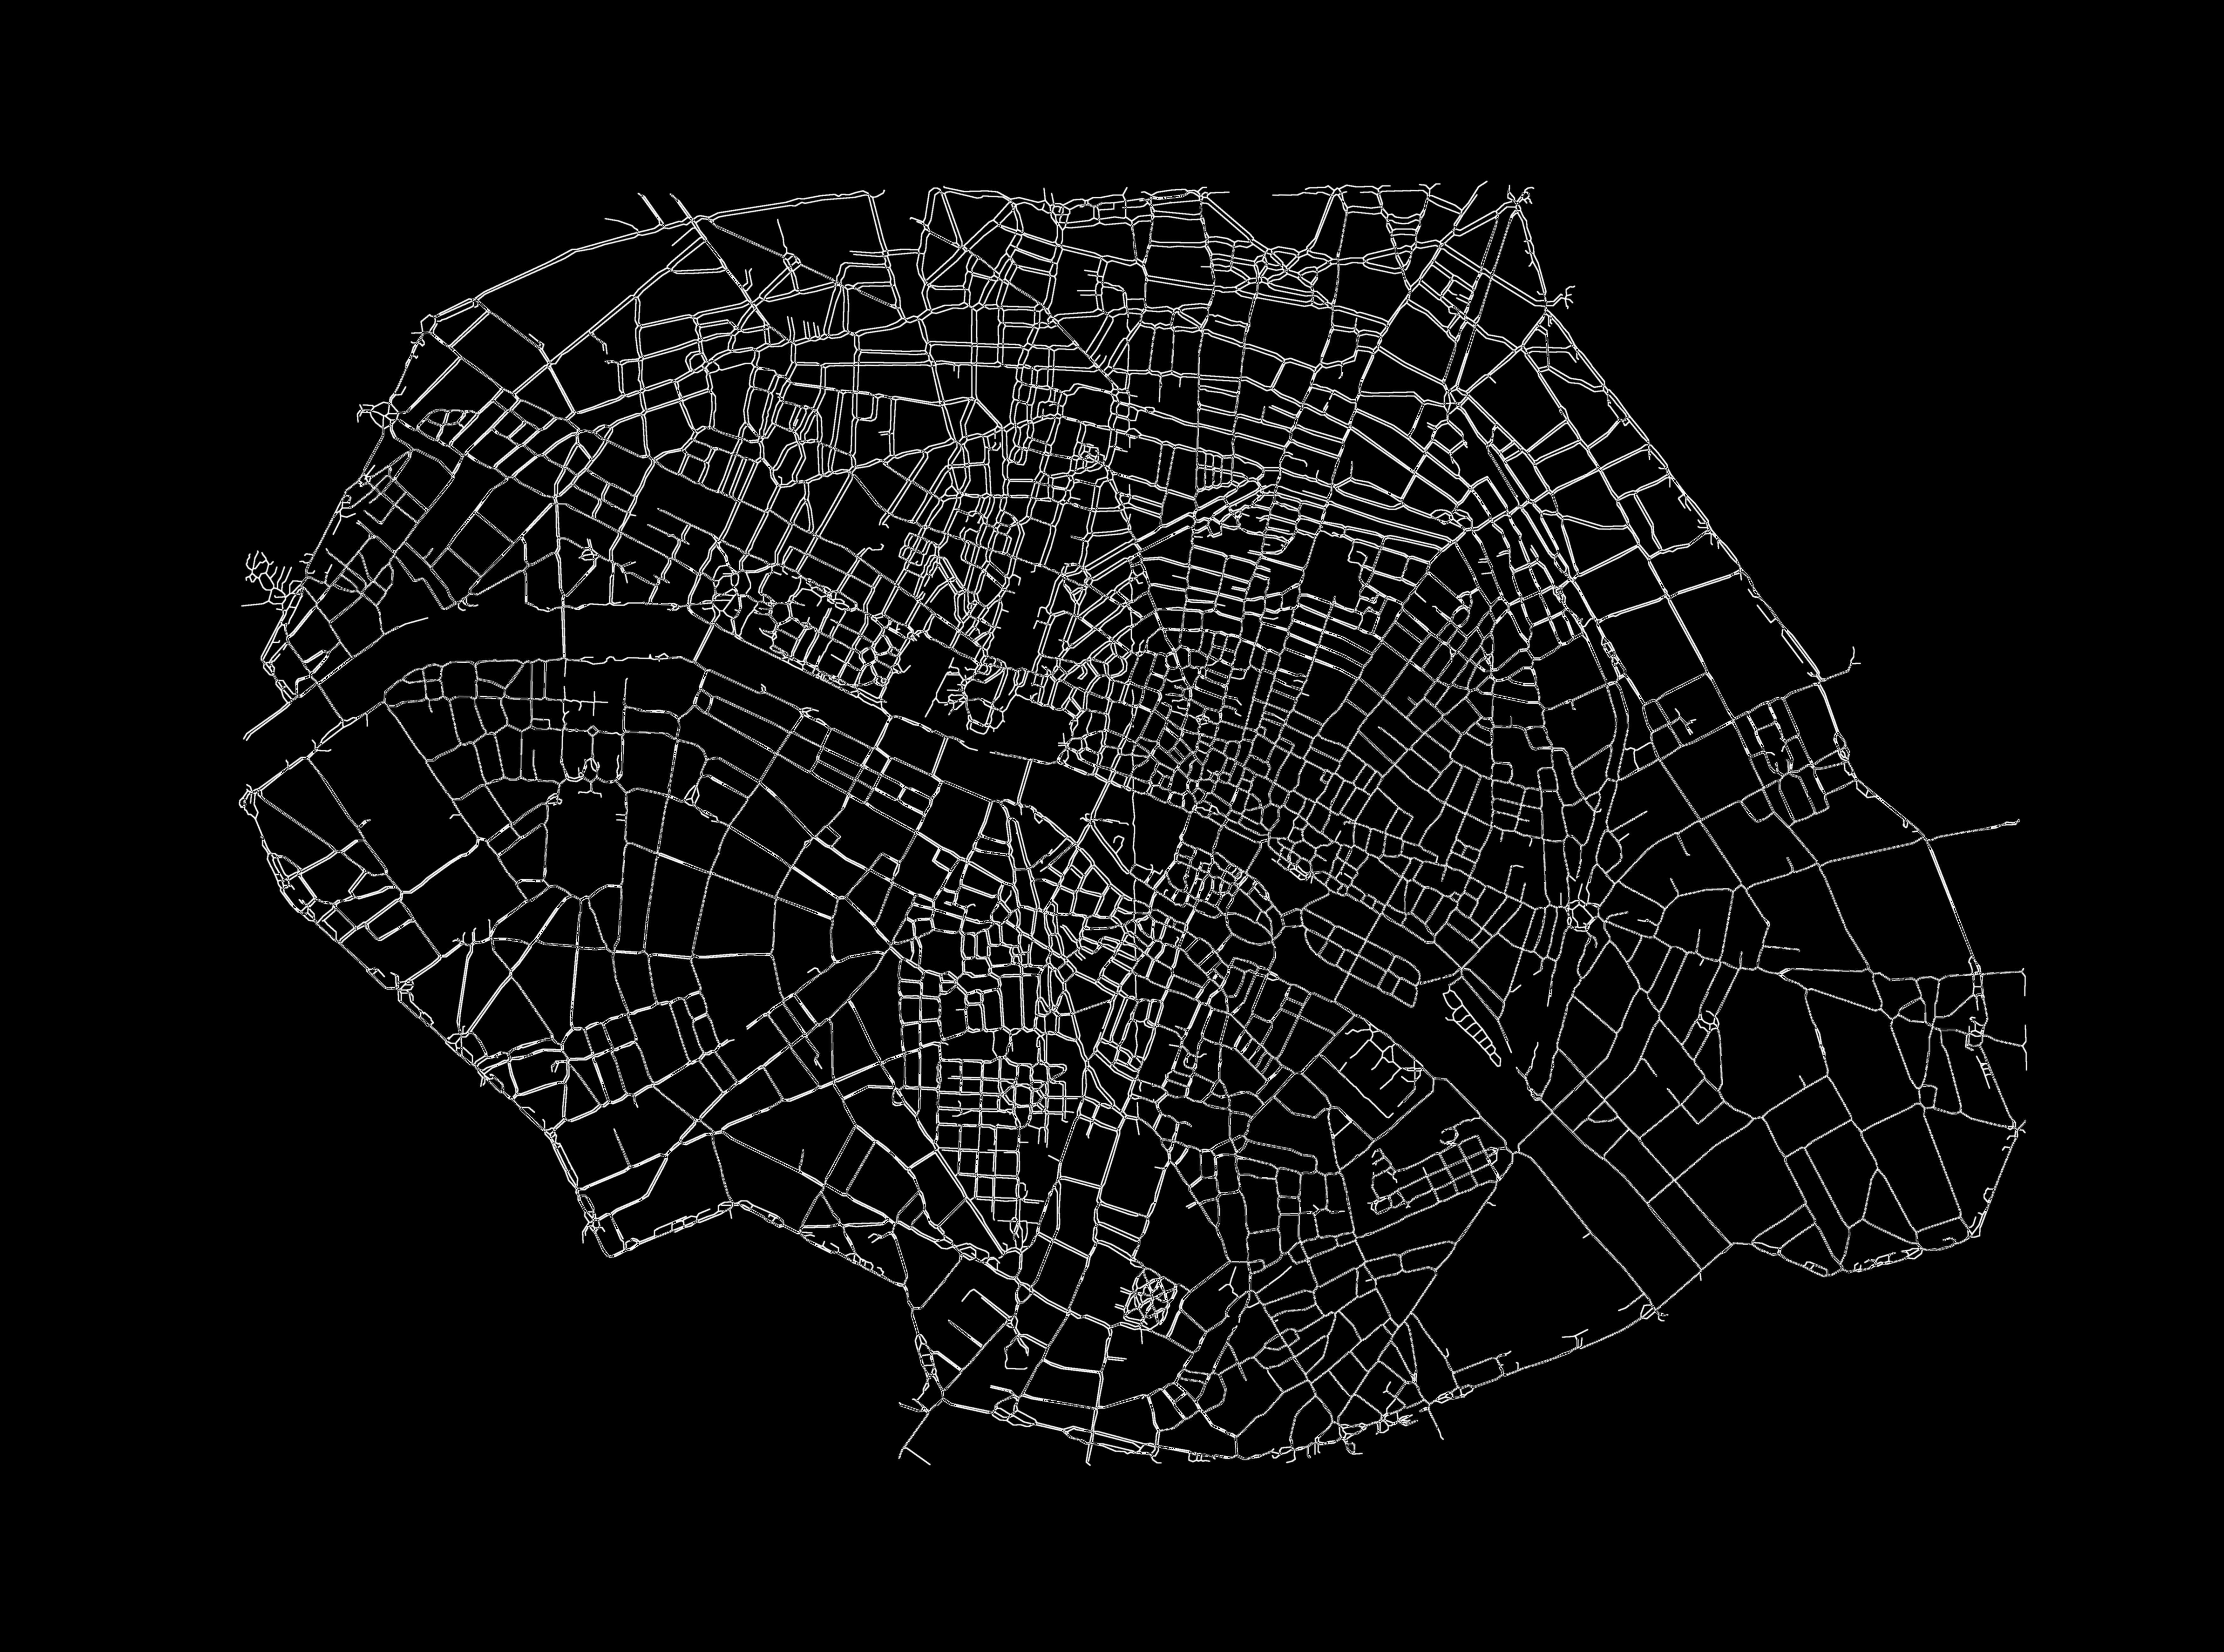
\includegraphics[width=0.9\textwidth]{Images/Map1/map_1_allignment_radius_110.png}
\caption{Alignment result of the alignment alrorithm with ORB}
\label{orb1}
\end{figure}

\begin{figure}[h!]
\centering
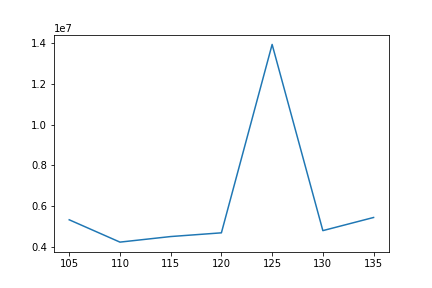
\includegraphics[width=0.6\textwidth]{Images/Map1/similarity_versus_radius_map_1.png}
\caption{Plot of the number of active pixels in the overlapped map versus search radius}
\label{search1}
\end{figure}

\begin{figure}[h!]
     \centering
     \begin{subfigure}{0.48\textwidth}
         \centering
         \includegraphics[width=\textwidth]{Images/Map1/map1_radius105.png}
         \caption{Search radius bring 105 pixels}
     \end{subfigure}
     \hfill
     \begin{subfigure}{0.48\textwidth}
         \centering
         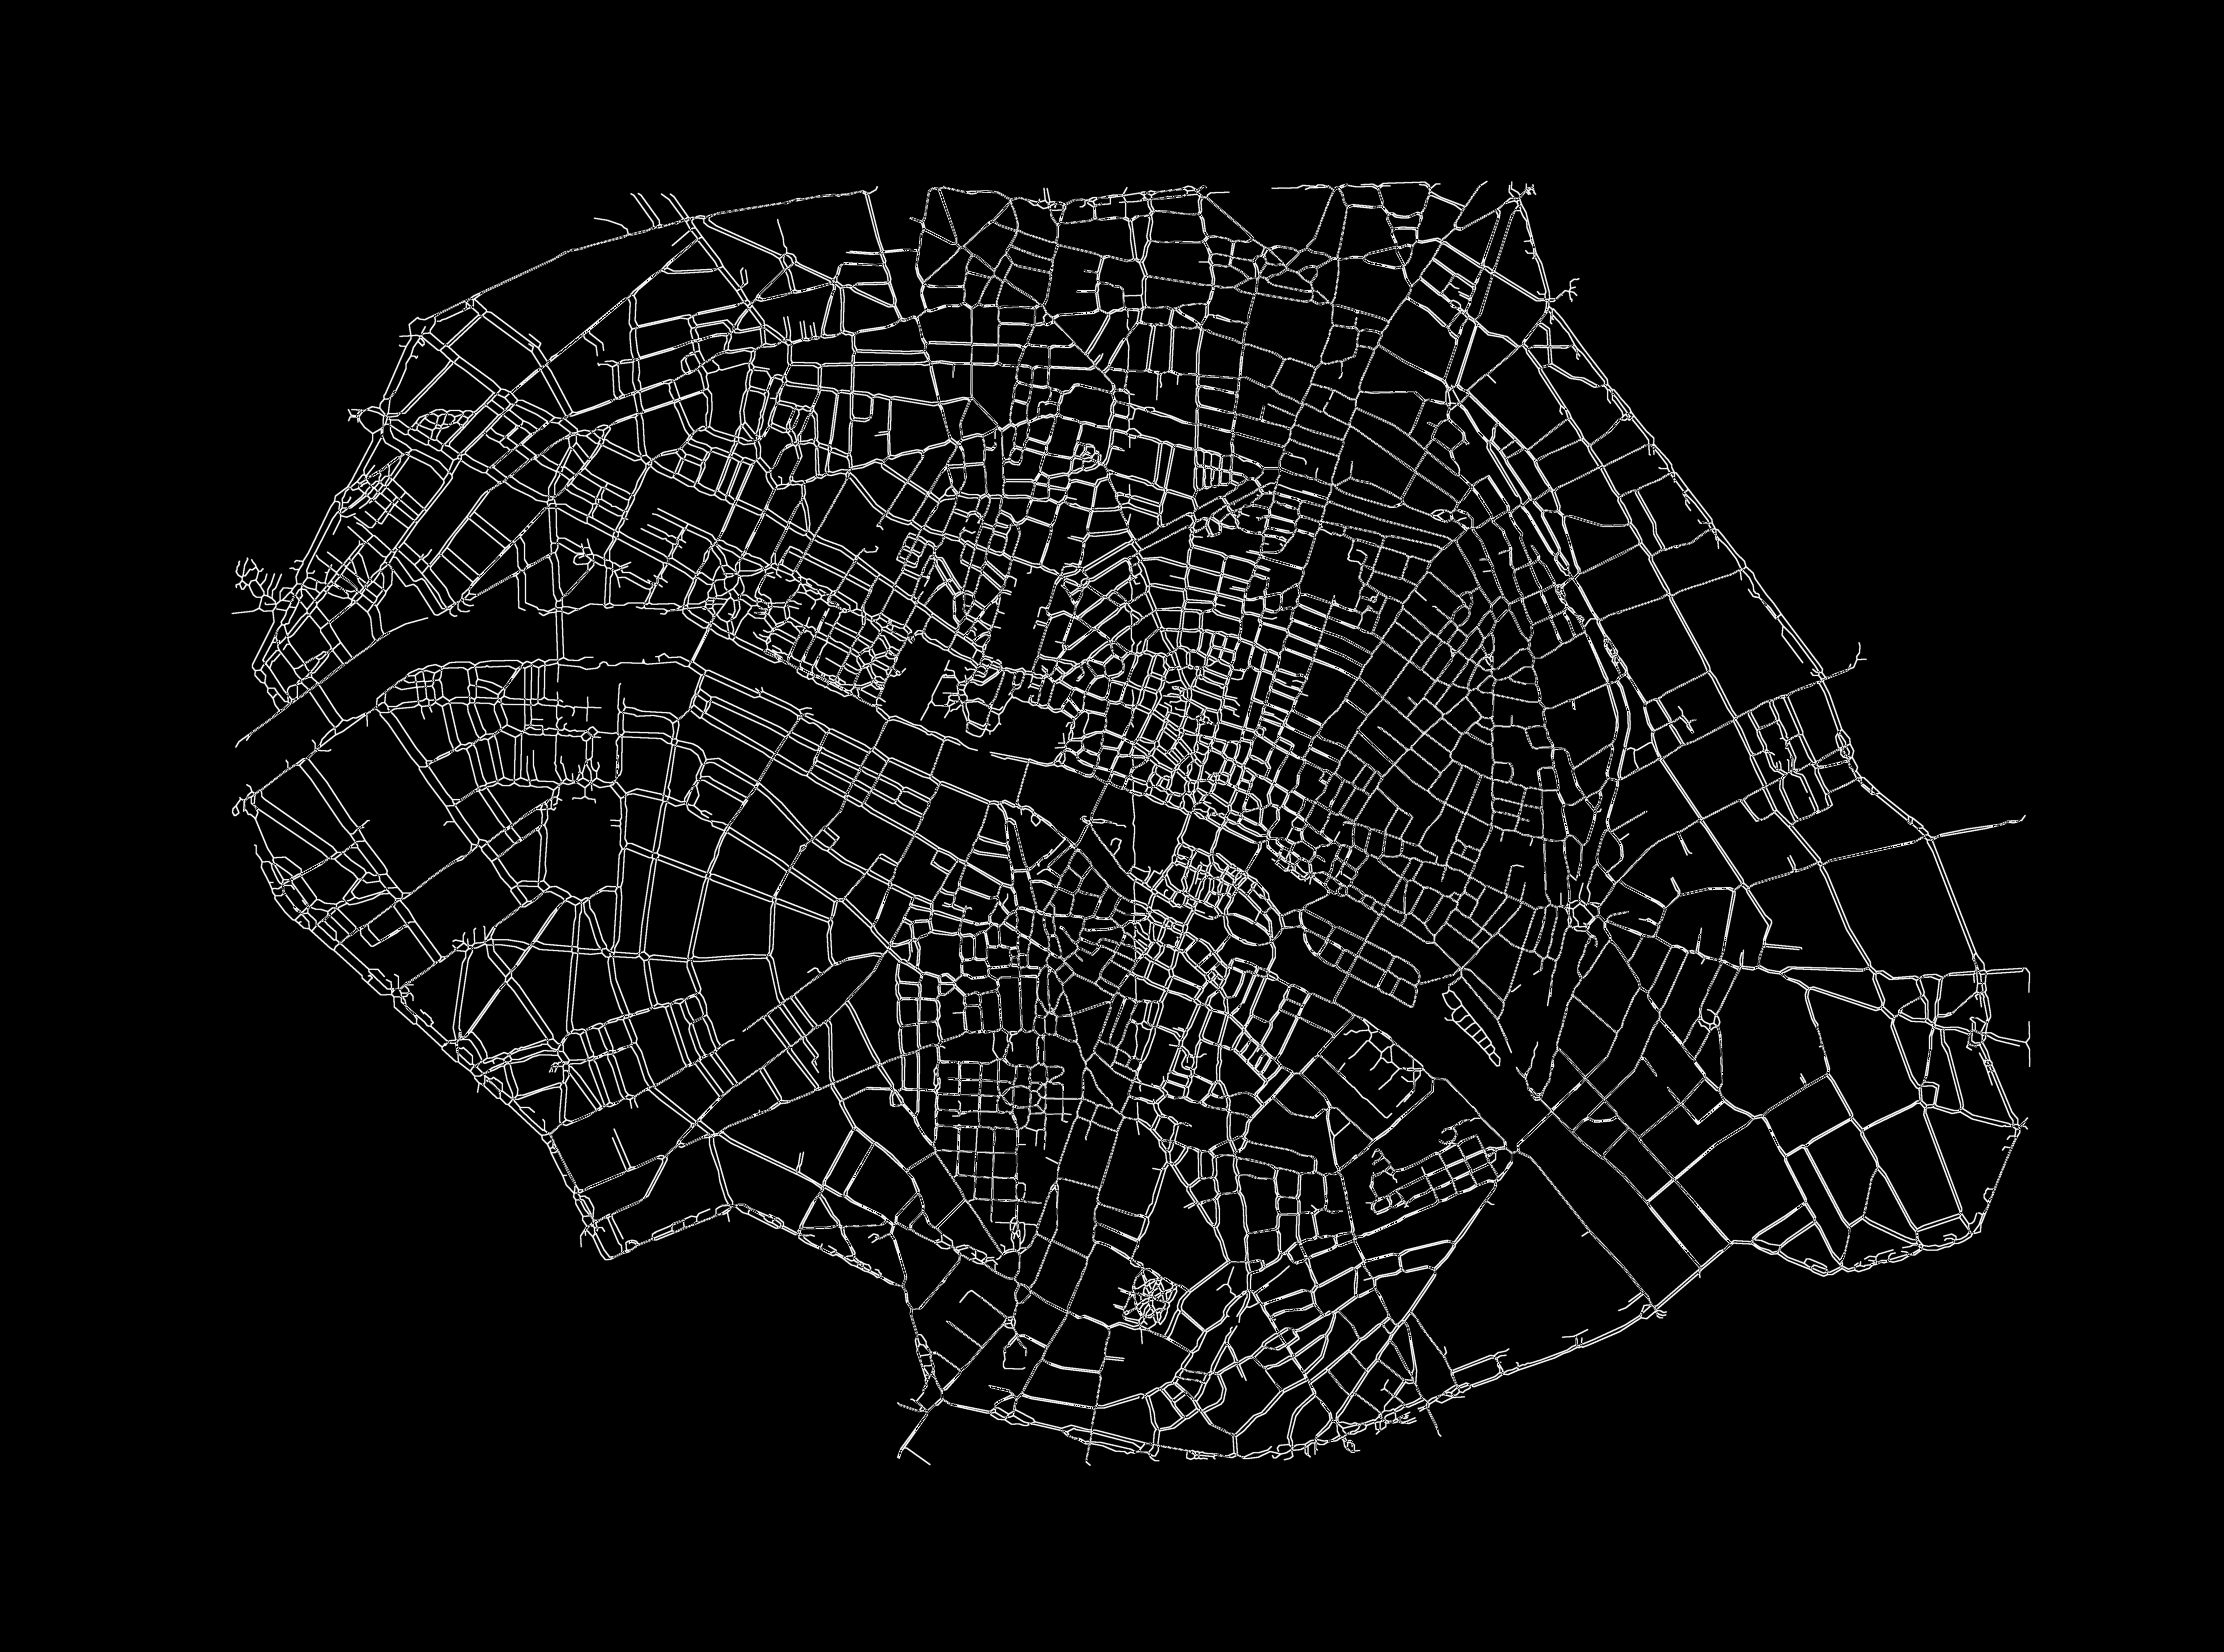
\includegraphics[width=\textwidth]{Images/Map1/map1_radius115.png}
         \caption{Search radius bring 115 pixels}
     \end{subfigure}
     \hfill
     \begin{subfigure}{0.48\textwidth}
         \centering
         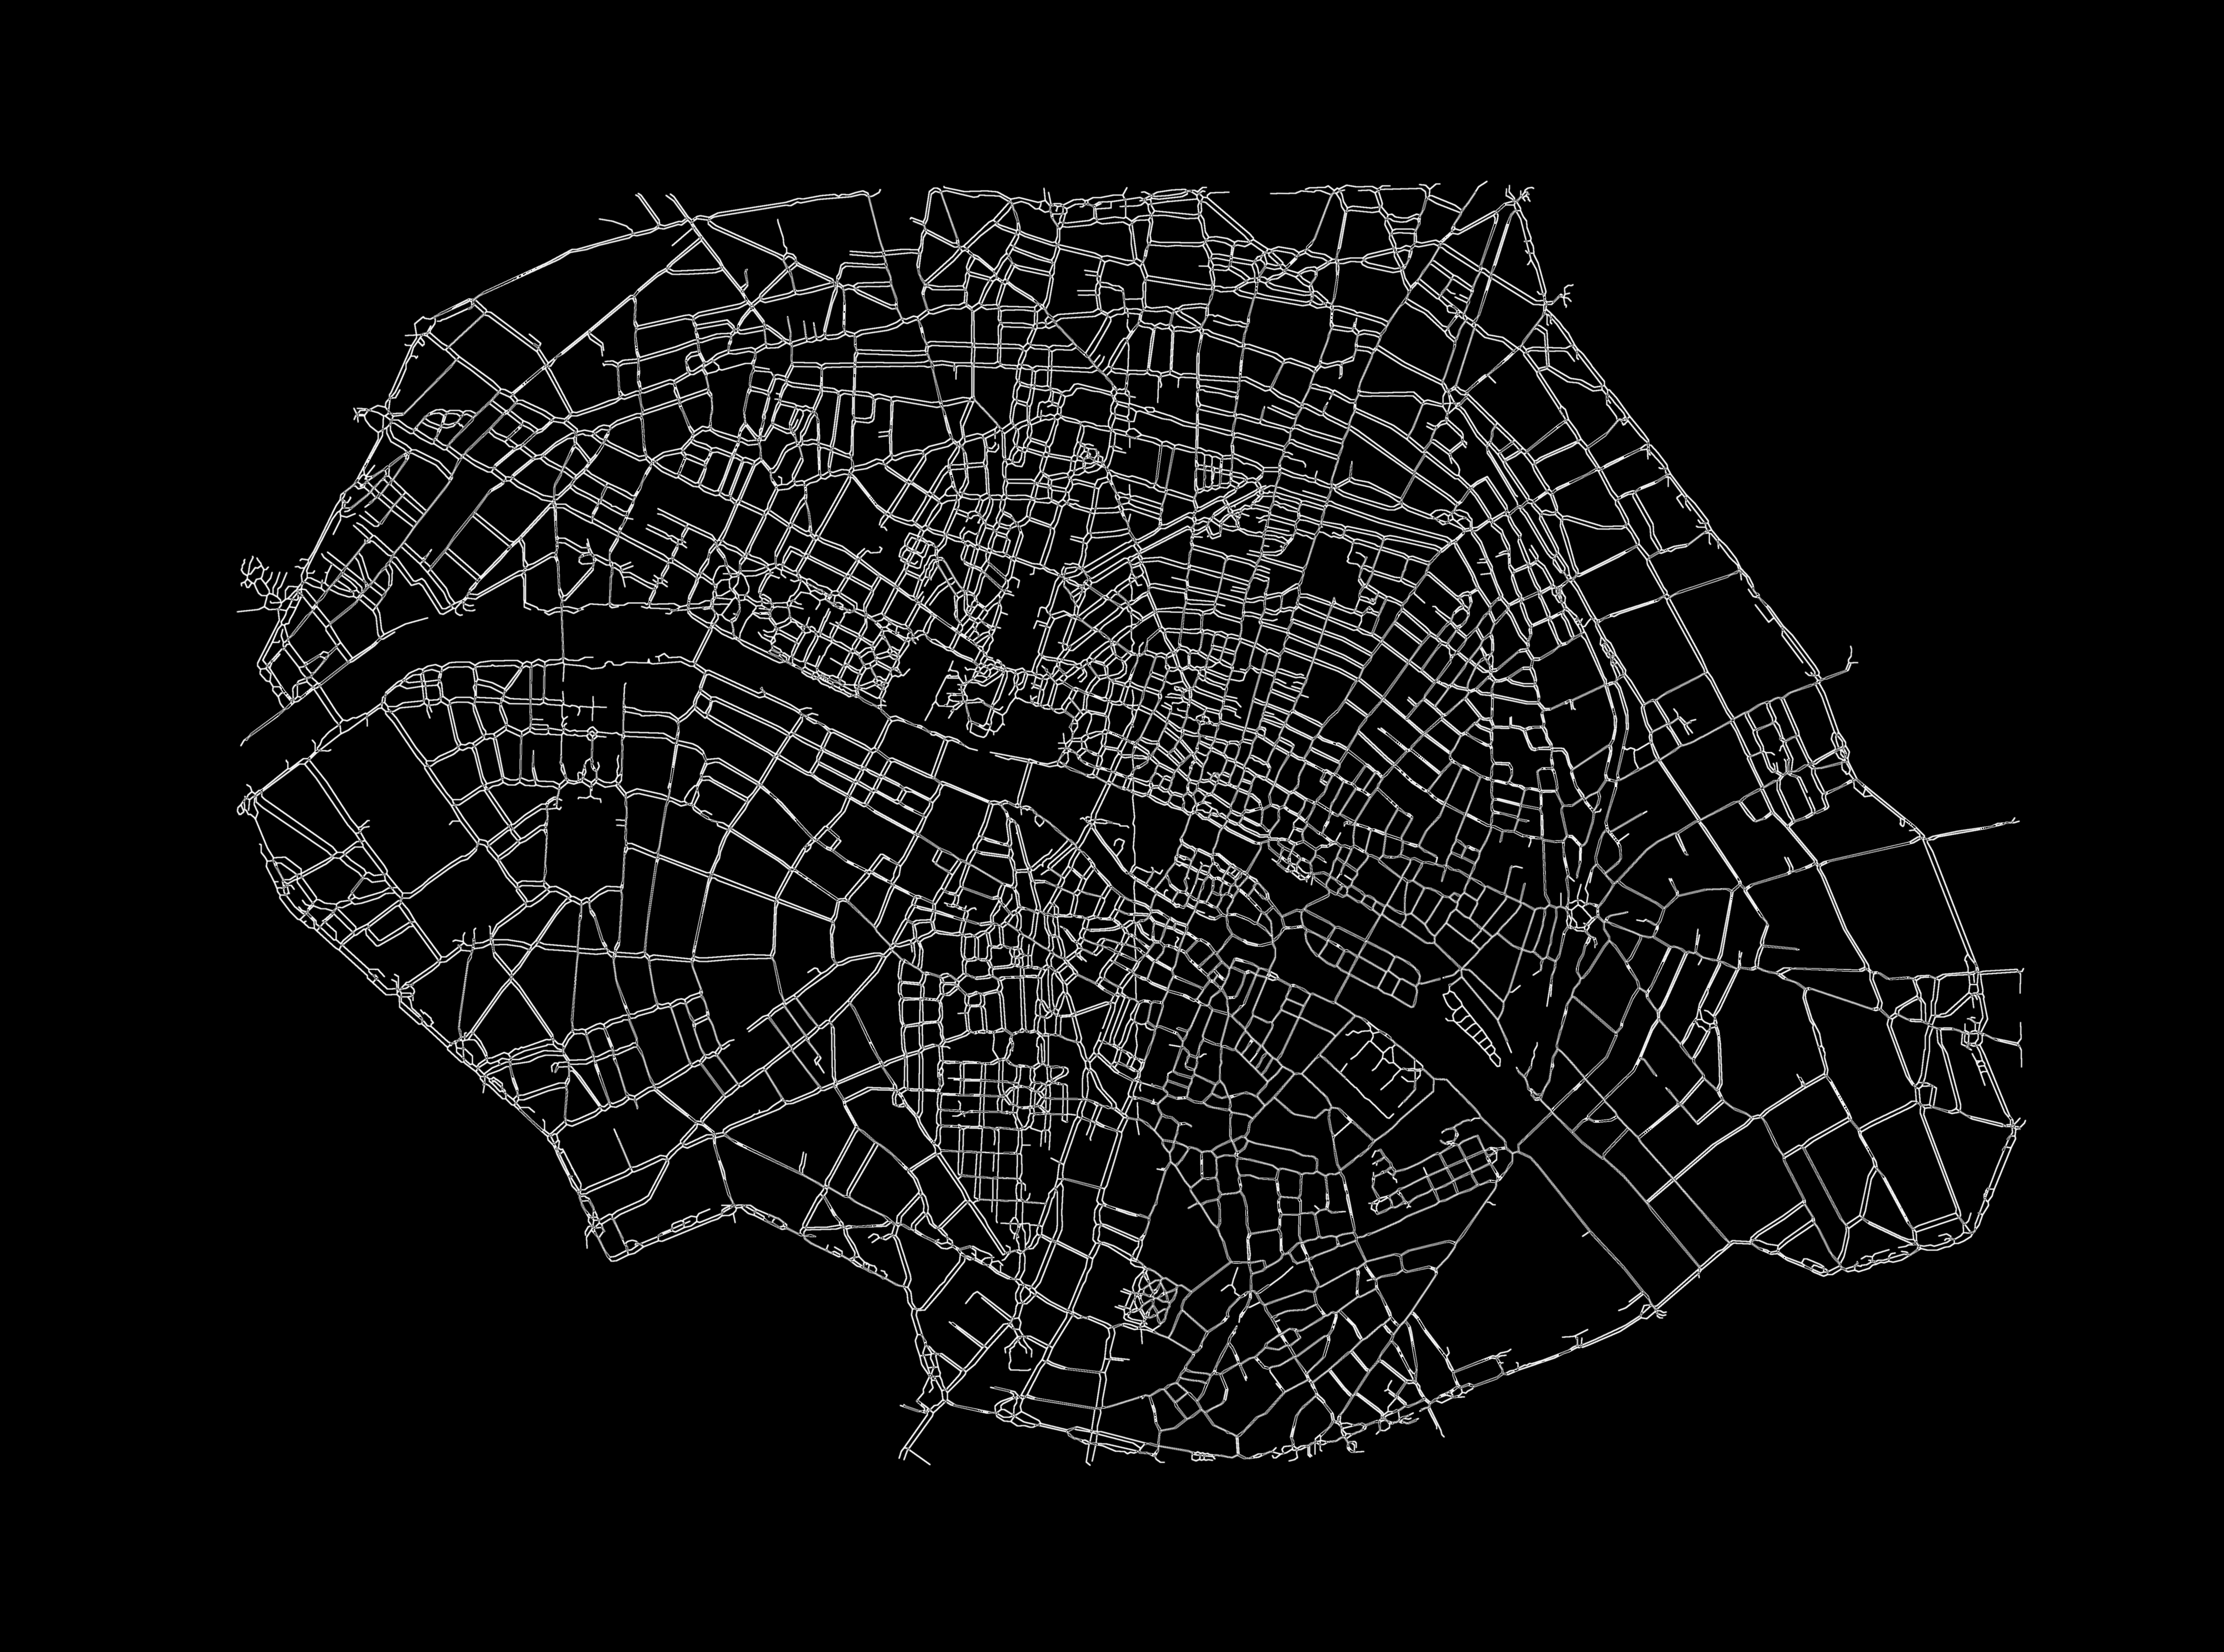
\includegraphics[width=\textwidth]{Images/Map1/map1_radius120.png}
         \caption{Search radius bring 120 pixels}
     \end{subfigure}
     \hfill
     \begin{subfigure}{0.48\textwidth}
         \centering
         \includegraphics[width=\textwidth]{Images/Map1/map1_radius125.png}
         \caption{Search radius bring 125 pixels}
     \end{subfigure}
     \hfill
     \begin{subfigure}{0.48\textwidth}
         \centering
         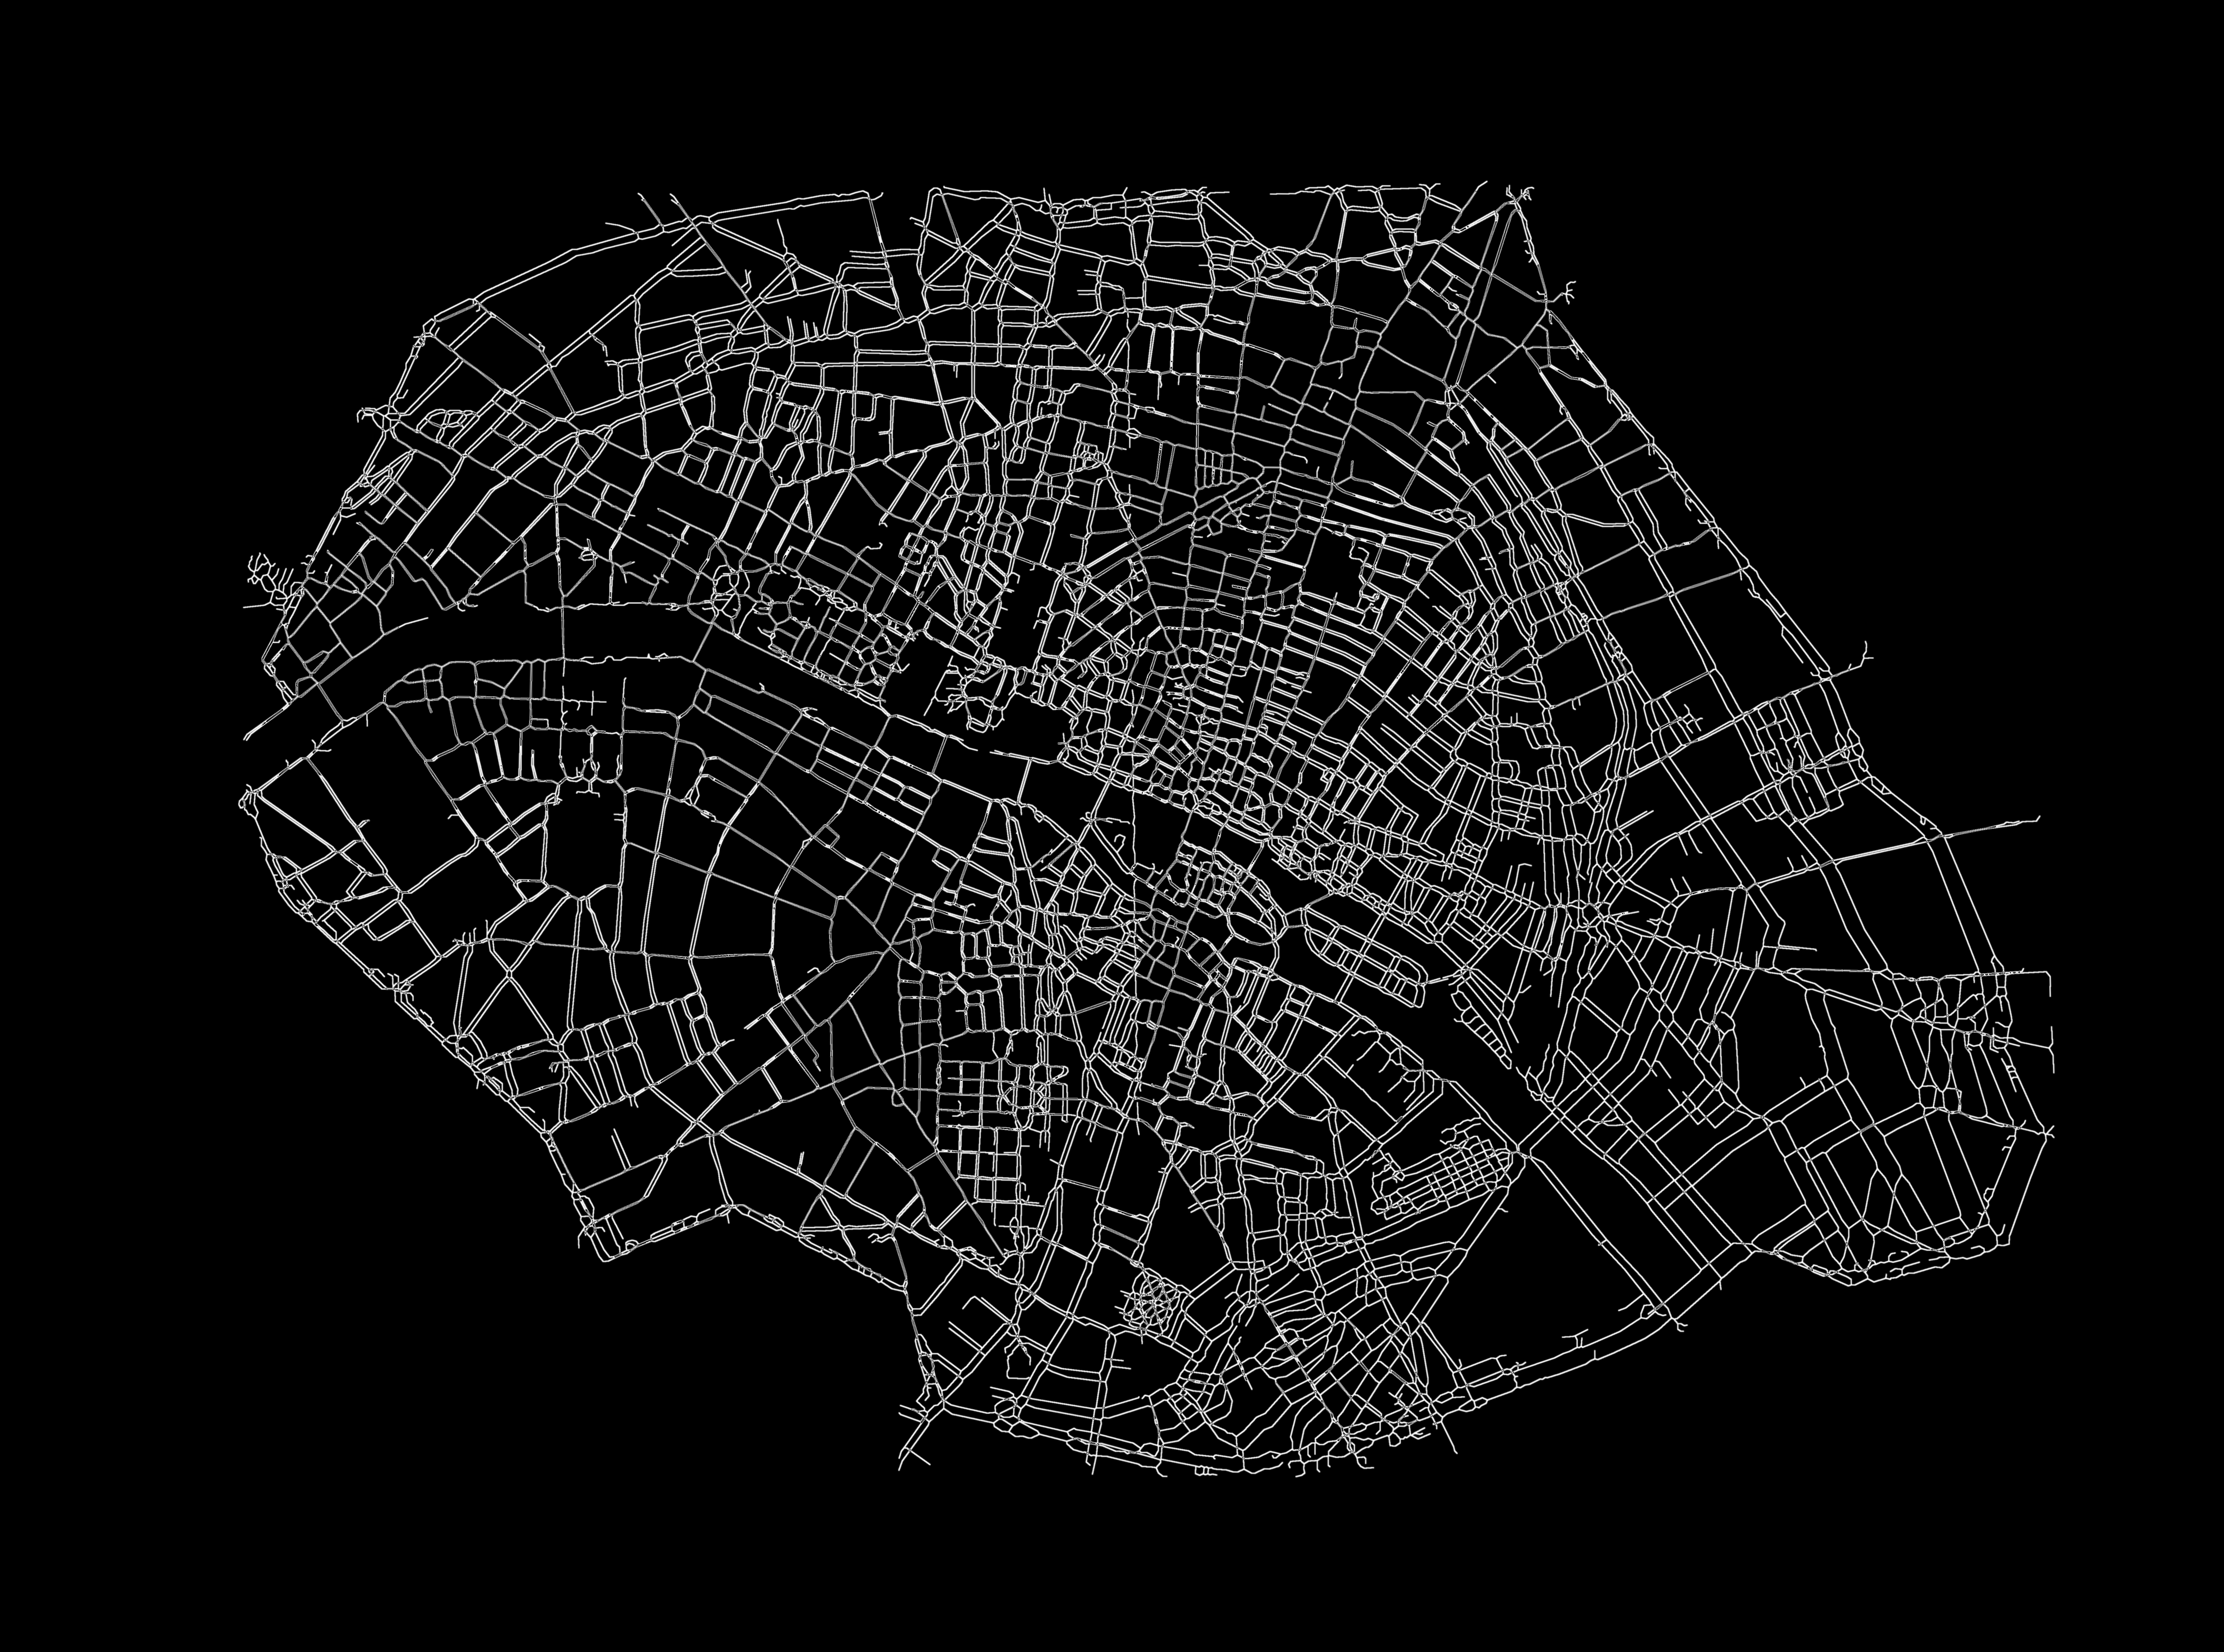
\includegraphics[width=\textwidth]{Images/Map1/map1_radius130.png}
         \caption{Search radius bring 130 pixels}
     \end{subfigure}
     \hfill
     \begin{subfigure}{0.48\textwidth}
         \centering
         \includegraphics[width=\textwidth]{Images/Map1/map1_radius135.png}
         \caption{Search radius bring 135 pixels}
     \end{subfigure}
        \caption{Alignment result with different search radius.}
        \label{orb1:other}
\end{figure}

However, the algorithm does not work all the time. The alignment result of \textit{Nouveau plan routier de la ville de Paris 1841} and some other maps published from 1839 to 1842 is shown in Figure \ref{orb2} and Figure \ref{orb3}. While Figure \ref{orb2} contains successful result and Figure \ref{orb3} contains failed result. The corresponding plots of the number of active pixels versus search radius are shown in Figure \ref{search2} and Figure \ref{search3}

\begin{figure}[h!]
     \centering
     \captionsetup{width=.9\textwidth, justification=centering}
     \begin{subfigure}{0.48\textwidth}
         \centering
         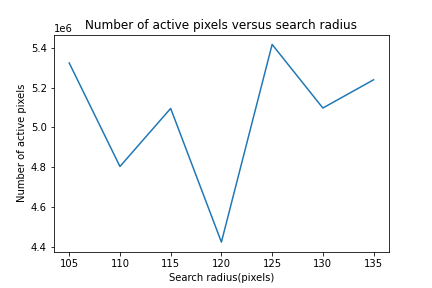
\includegraphics[width=\textwidth]{Images/Map other/similarity_versus_radius_map_7.png}
         \caption{\textit{Nouveau plan routier de la ville de Paris 1839}}
     \end{subfigure}
     \hfill
     \begin{subfigure}{0.48\textwidth}
         \centering
         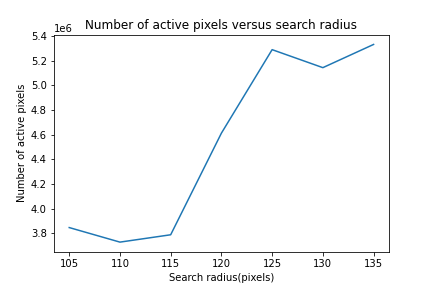
\includegraphics[width=\textwidth]{Images/Map other/similarity_versus_radius_map_10.png}
         \caption{\textit{Nouveau plan routier de la ville de Paris 1840}}
     \end{subfigure}
        \caption{Plot of the number of active pixels versus search radius of alignment in Figure \ref{orb2}, each plot is labeled by the other map name}
        \label{search2}
\end{figure}

\begin{figure}[h!]
     \centering
     \captionsetup{width=.9\textwidth, justification=centering}
     \begin{subfigure}{0.48\textwidth}
         \centering
         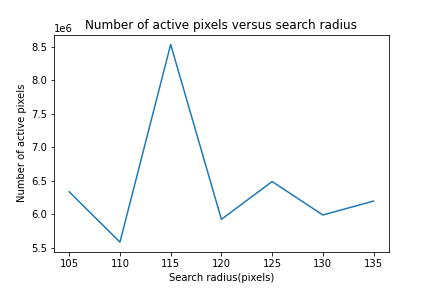
\includegraphics[width=\textwidth]{Images/Map other/similarity_versus_radius_map_13.png}
         \caption{\textit{Plan itinéraire et administratif de la ville de Paris 1839}}
     \end{subfigure}
     \hfill
     \begin{subfigure}{0.48\textwidth}
         \centering
         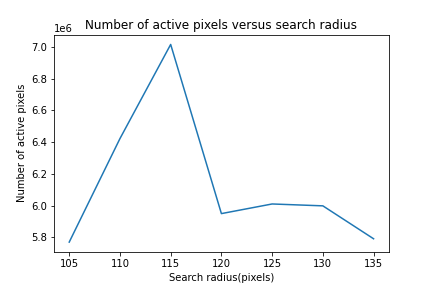
\includegraphics[width=\textwidth]{Images/Map other/similarity_versus_radius_map_22.png}
         \caption{\textit{Plan de Paris 1842}}
     \end{subfigure}
        \caption{Plot of the number of active pixels versus search radius of alignment in Figure \ref{orb3}, each plot is labeled by the other map name}
        \label{search3}
\end{figure}

\begin{figure}[h!]
     \centering
     \captionsetup{width=.9\textwidth, justification=centering}
     \begin{subfigure}{0.9\textwidth}
         \centering
         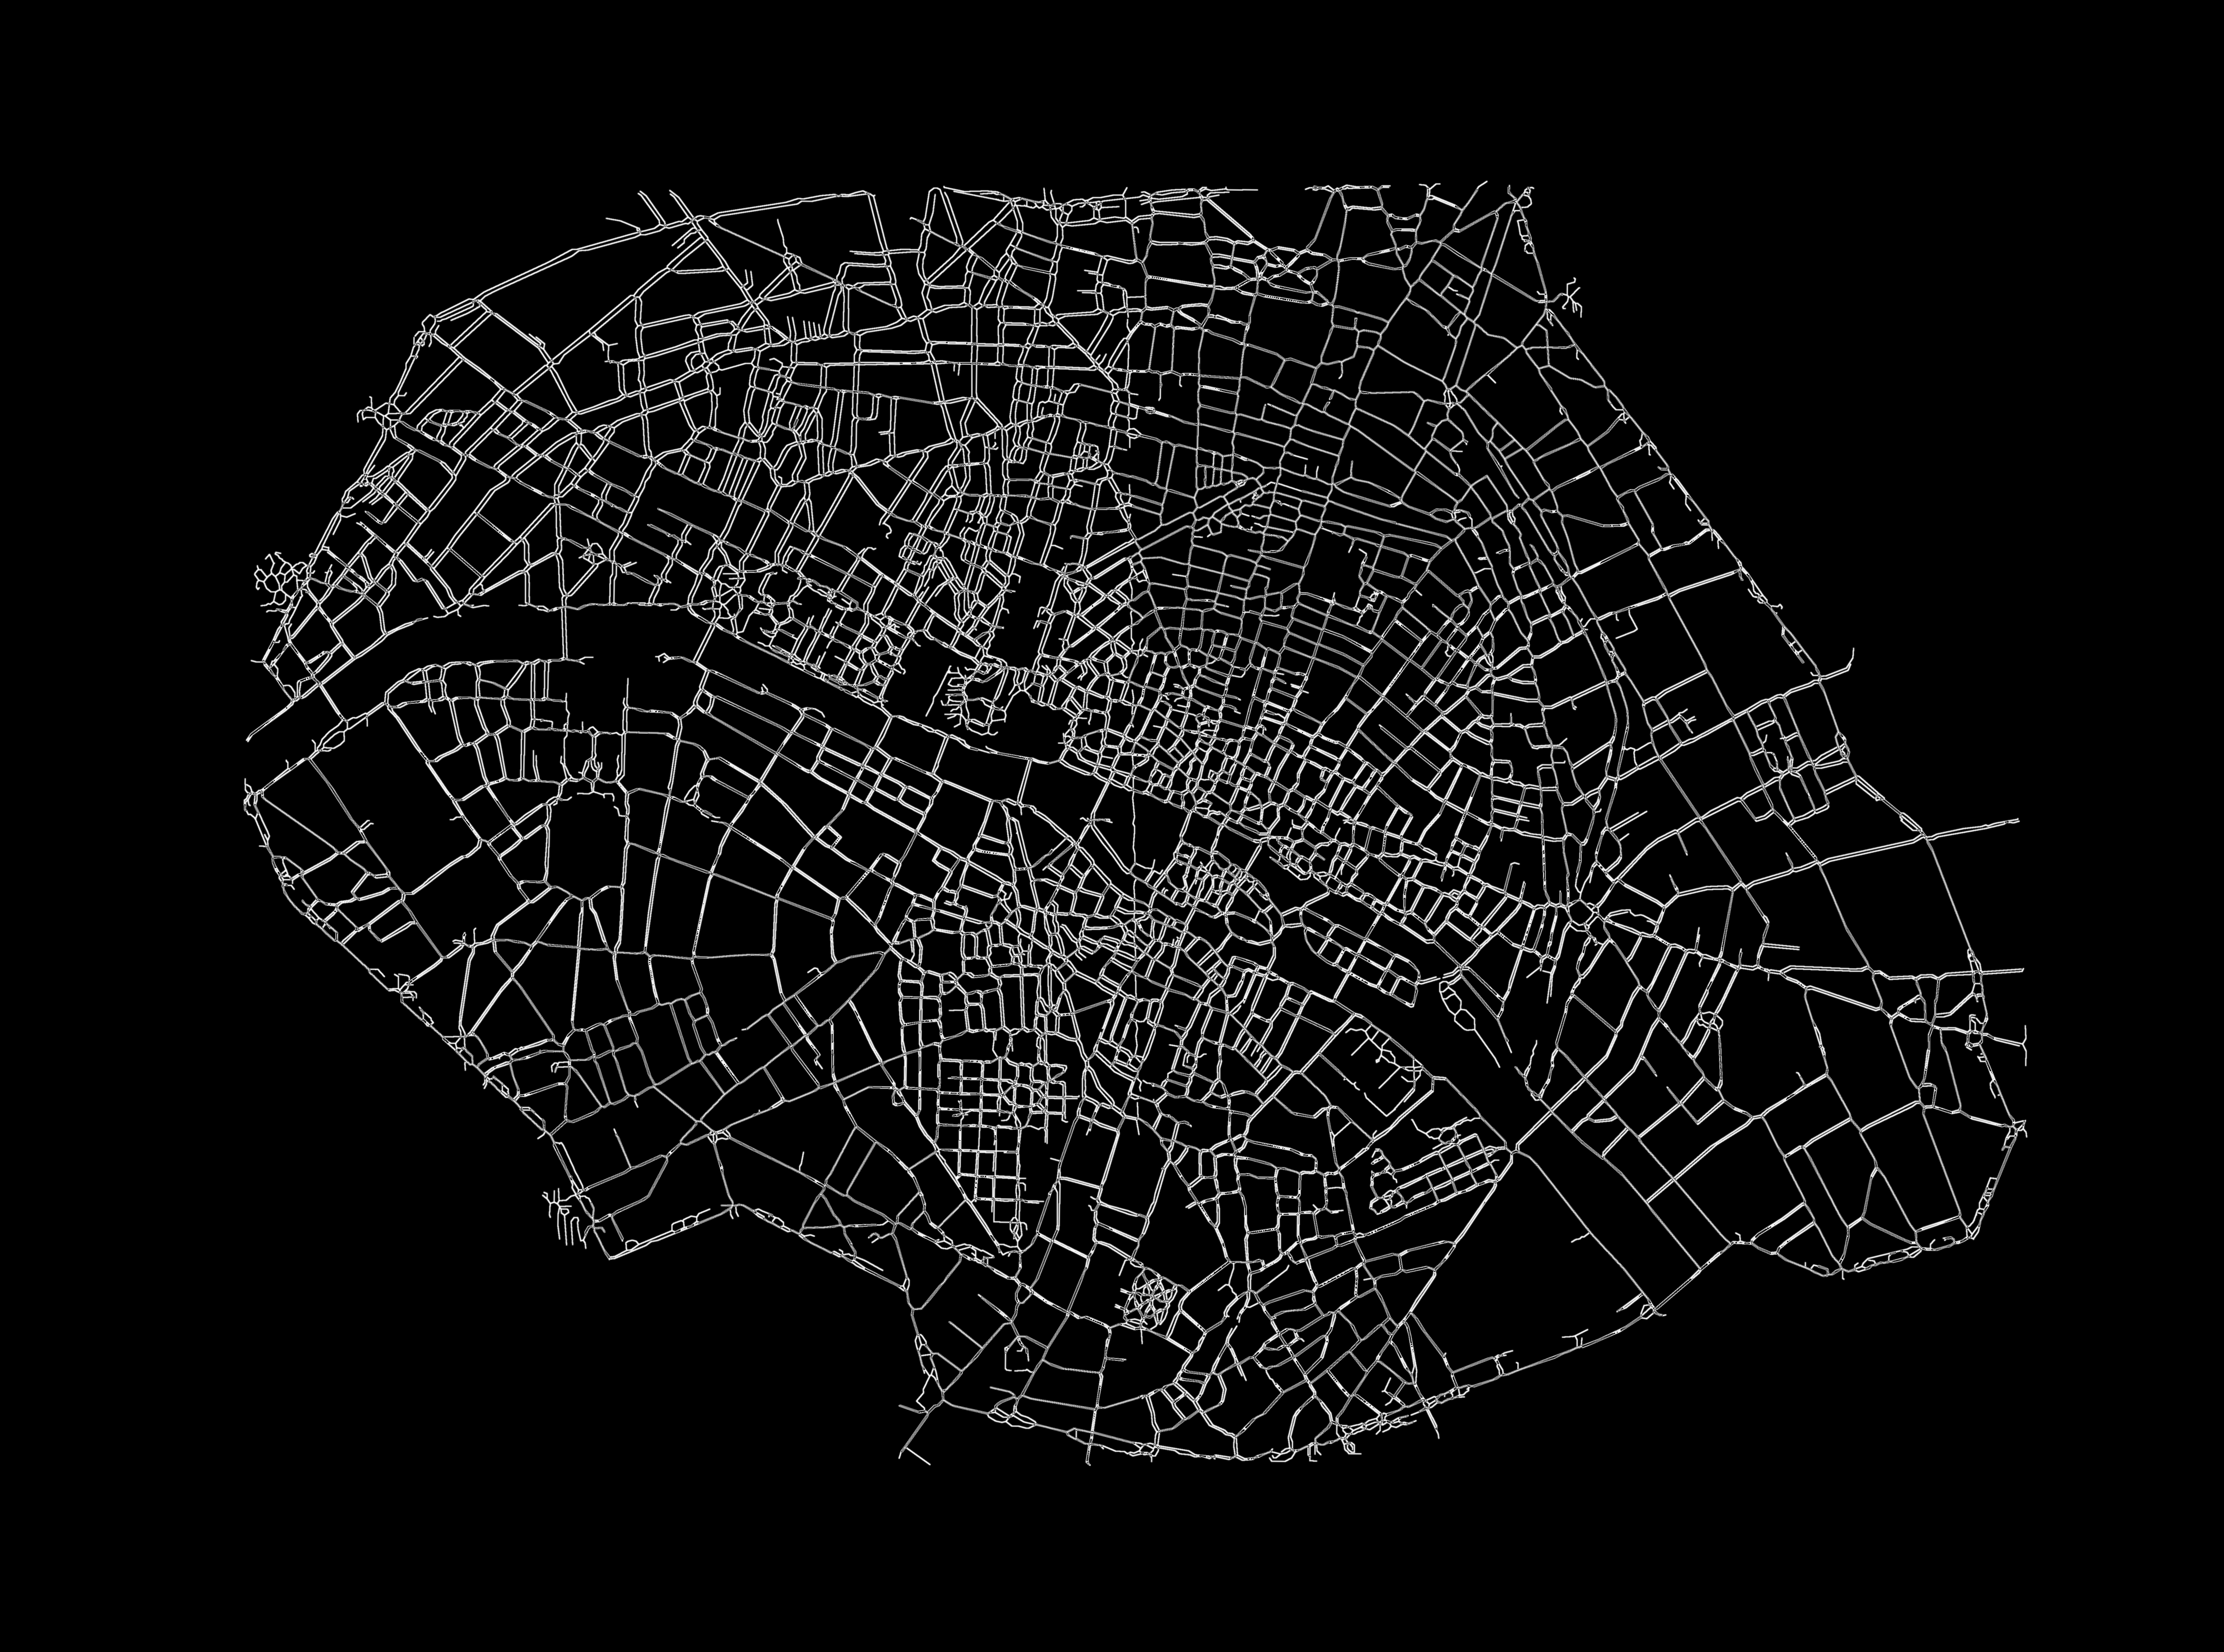
\includegraphics[width=\textwidth]{Images/Map other/map_7_allignment_radius_120.png}
         \caption{\textit{Nouveau plan routier de la ville de Paris 1839}}
     \end{subfigure}
     \hfill
     \begin{subfigure}{0.9\textwidth}
         \centering
         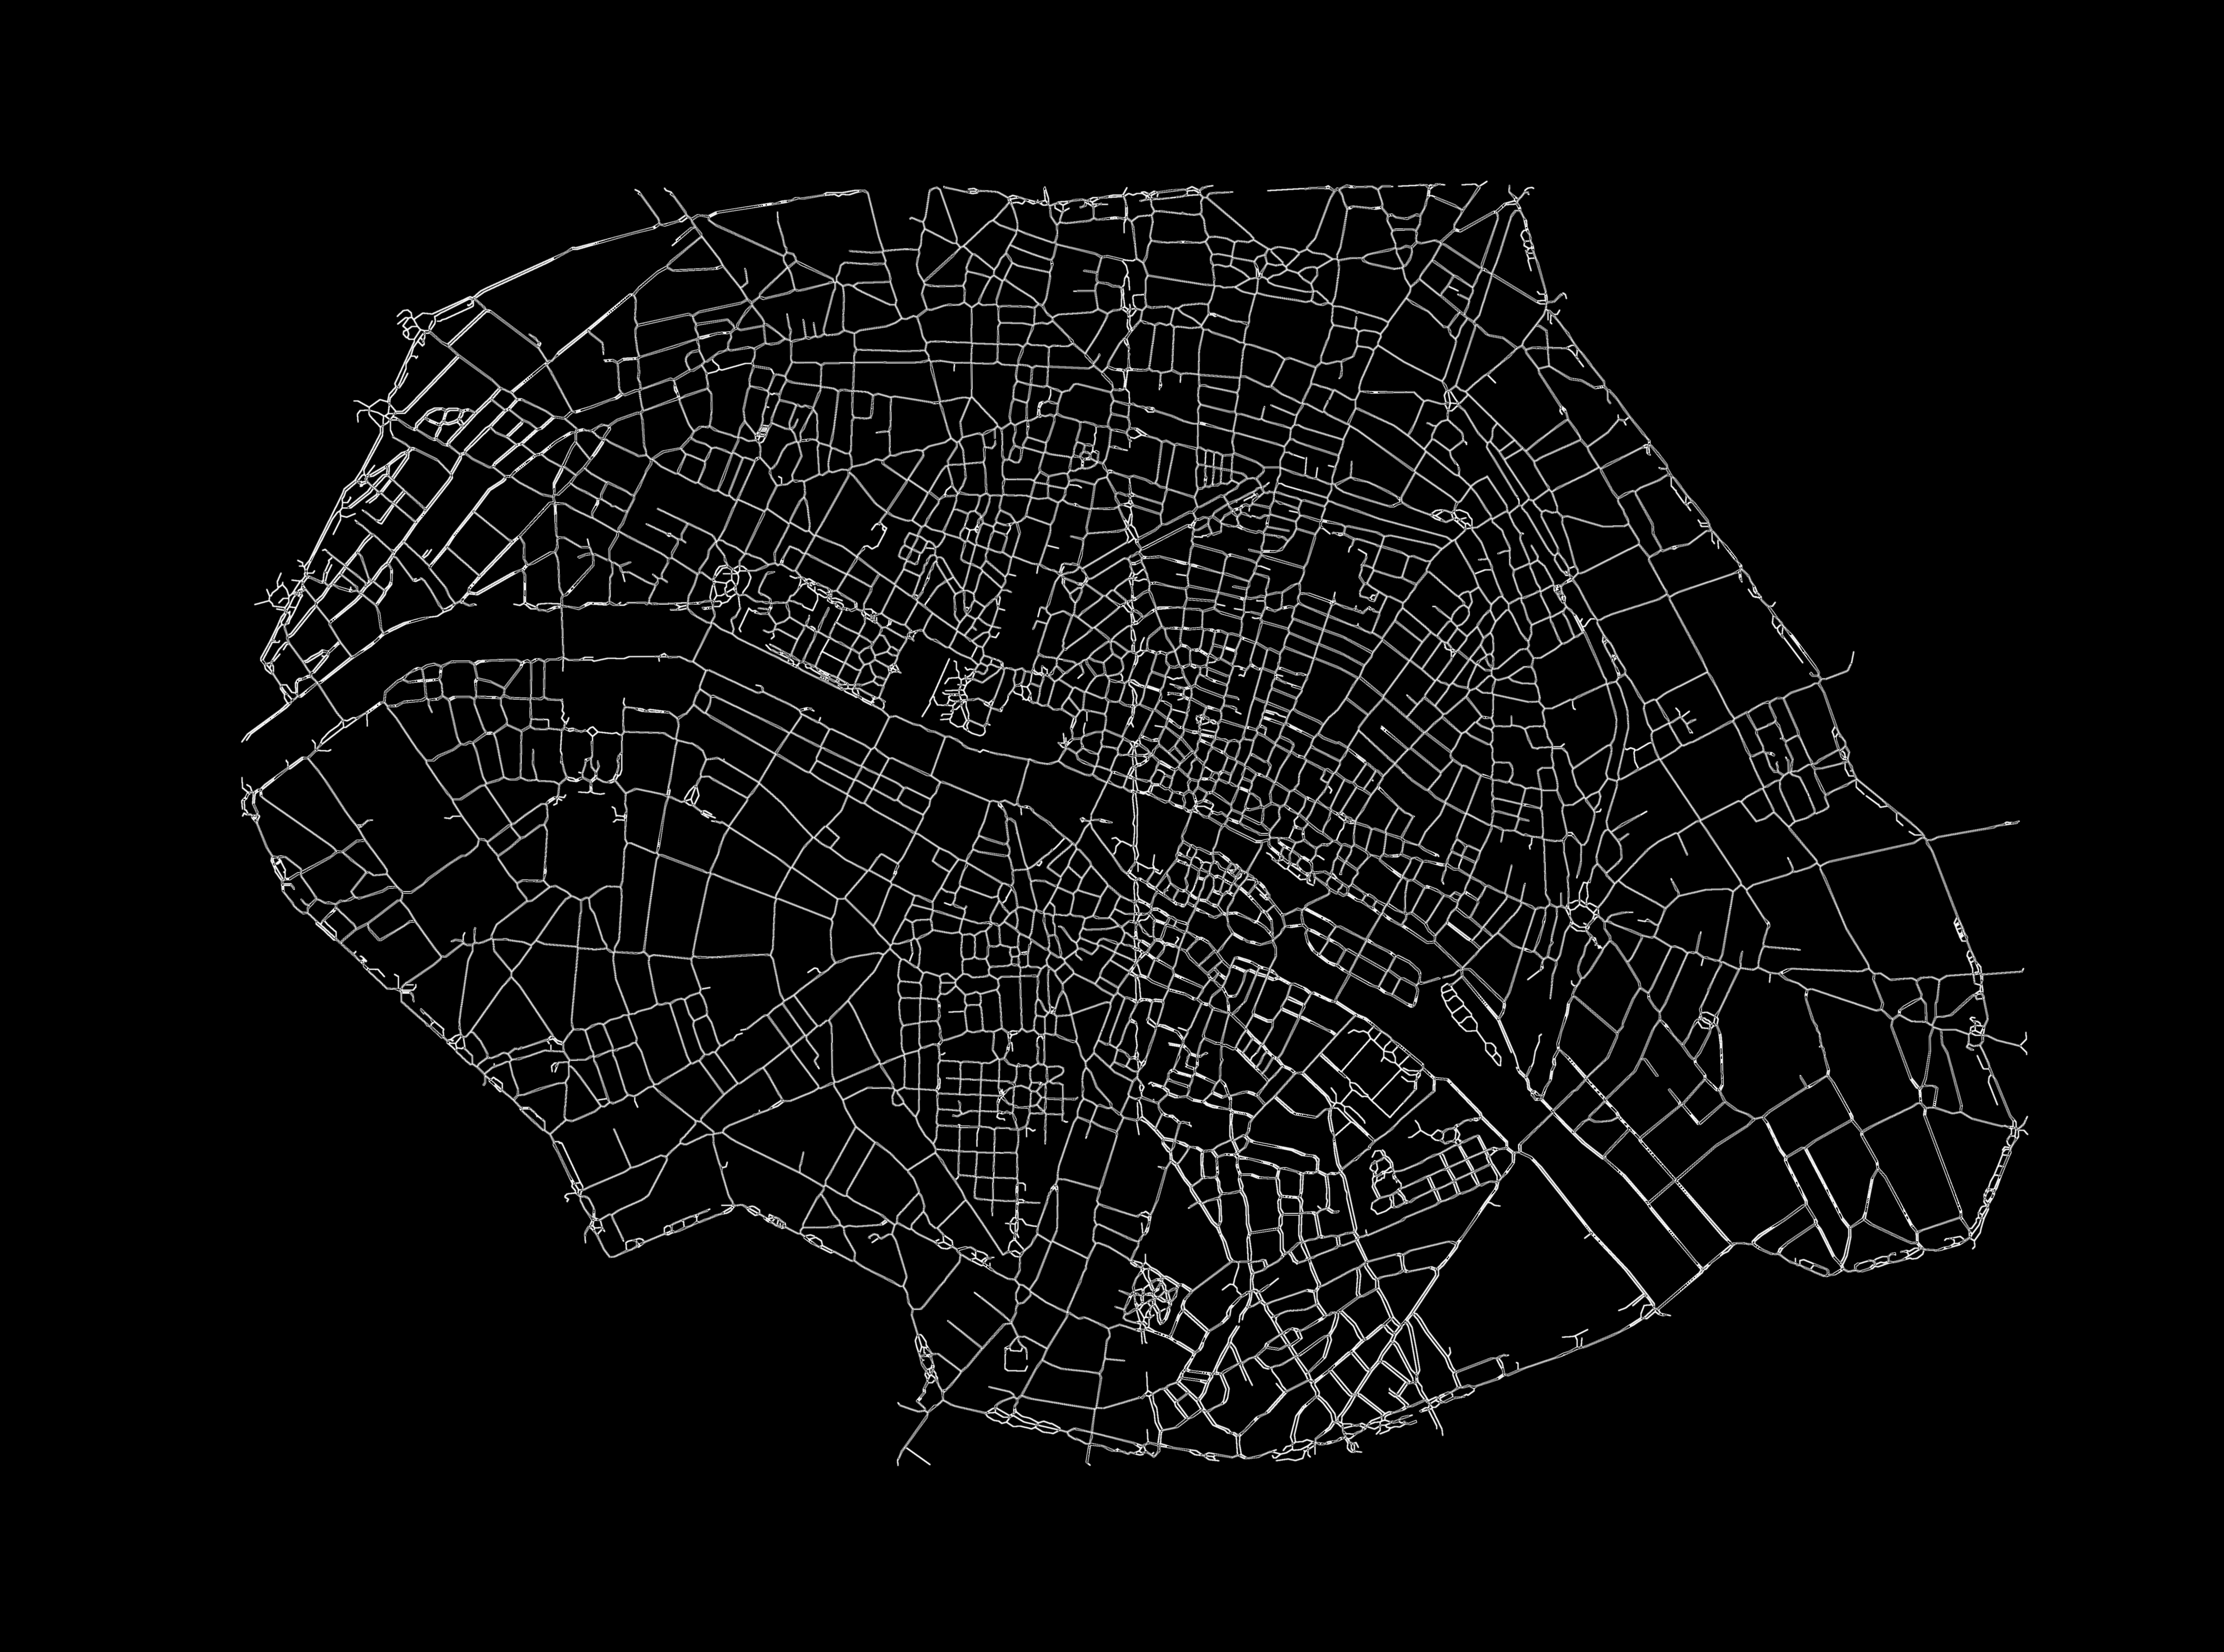
\includegraphics[width=\textwidth]{Images/Map other/map_10_allignment_radius_110.png}
         \caption{\textit{Nouveau plan routier de la ville de Paris 1840}}
     \end{subfigure}
        \caption{Successful result of other maps aligned to \textit{Nouveau plan routier de la ville de Paris 1841}, each plot is labeled by the other map name}
        \label{orb2}
\end{figure}

\begin{figure}[h!]
     \centering
     \captionsetup{width=.9\textwidth, justification=centering}
     \begin{subfigure}{0.9\textwidth}
         \centering
         \includegraphics[width=\textwidth]{Images/Map other/map_13_allignment_radius_110.png}
         \caption{\textit{Plan itinéraire et administratif de la ville de Paris 1839}}
     \end{subfigure}
     \hfill
     \begin{subfigure}{0.9\textwidth}
         \centering
         \includegraphics[width=\textwidth]{Images/Map other/map_22_allignment_radius_105.png}
         \caption{\textit{Plan de Paris 1842}}
     \end{subfigure}
        \caption{Failed result of other maps aligned to \textit{Nouveau plan routier de la ville de Paris 1841}, each plot is labeled by the other map name}
        \label{orb3}
\end{figure}


Overall, compared with the ECC maximization algorithm discussed in section \ref{ecc_result}, the alignment algorithm with ORB improves the alignment result 50\% of the time.

% If the maps are not dilated and Gaussian smoothed, the alignment result is shown in Figure \ref{noprocess}. Same maps in section \ref{ecc_result} are used. To better visualize the result, the final aligned map are dilated and Gaussian smoothed.

The unit of the search radius is pixels. For this experiment, 10000 pixels is equivalent to \ang{0;7;6.826} in latitude and \ang{0;10;44.26} in longitude.

\subsection{Discussion}

If the corresponding feature points detected by ORB are successfully matched, as in Figure \ref{orb1} and \ref{orb2}, this algorithm can perfectly align two maps. However, we find out the algorithm only works 50\% percent of the time. From Figure \ref{orb3} and \ref{search3}, it might be because we only test the search radius within 105 pixels and 135 pixels. Compare Figure \ref{orb2} and Figure \ref{orb3}, the algorithm also performs better when two maps have a similar shape or structure.

As the ECC Maximization algorithm improves the alignment algorithm for all the maps, we can use the algorithm in this section as a supplement to further improve the alignment if possible.

For this project, we align the maps published in the same period to get the ground truth map of Paris, which usually has similar content and structure. Therefore, the shortcomings of this algorithm are weakened in this project.

There are two other parameters that affect the performance of the algorithm greatly:

\subsubsection{Search radius}

Search radius greatly affects the performance of the algorithm. As illustrated in Figure \ref{orb1:other} and \ref{search1}. With a large search radius, points may be mapped to other unreasonable key points that are far away from themselves. With a small search radius, because of the misalignment, points may not be mapped to the key points representing the same place on another map. Ideally, the search radius should be defined in degree, the same as latitude and longitude. In this case, the scale of the map or the canvas size will not affect the choice of the search radius. 

There is no global choice of search radius that works for all. It is highly dependent on how misaligned two maps are. In this algorithm, we set a reference search radius, and the algorithm would use the best search radius it can find around this reference.

The performance of the search radius is measured by the number of active pixels of the overlapped map of $A$ and $B$. A pixel is active if it is not of value 0. Denote number of active pixels of $A$, $B$, overlapped map as $p_A$, $p_B$ and $p_\text{overlap}$ respectively. In the ideal case, if $A$ and $B$ can be perfectly aligned, $p_\text{overlap}$ would be close to $p_A$. Otherwise, the overlapped map would have more active pixels. In the extreme case where $A$ and $B$ are not aligned at all, $p_\text{overlap}$ would be close to $p_A+p_B$.

% The map alignment examples and their best locally search radius is showed in Figure \ref{radius2}

This quantification method is proved by Figure \ref{orb1}, \ref{search1} and \ref{orb2}. The search radius with the lowest number of active pixels does have the best alignment result.

\subsubsection{Dilation and Gaussian smoothing}
The vectorized map is mathematically a binary matrix. It turns out that ORB usually fails to detect the feature point of such kind of image. We find out that with the same search radius, the map being dilated and smoothed has a better alignment result.

% \section{Density of the road pixels}

% Density of the road pixels is one indication of the urbanization of a area.

% Check and align the time period with more than 5 aligned maps and count the number of road pixels within.